\documentclass[reqno]{amsart}

\usepackage{amsfonts,latexsym,amsthm,amssymb,amsmath,amscd,euscript,bm}
\usepackage[sc]{mathpazo}
\usepackage[margin = 2.6cm]{geometry}
\usepackage{enumitem}
\usepackage{graphicx}
\usepackage{hyperref}
% sets numbering of enumerate to a, b, c, ...
\renewcommand{\theenumi}{\alph{enumi}}

% Theorems, propositions, etc.
\newtheorem{theorem}{Theorem}
\newtheorem{proposition}[theorem]{Proposition}
\newtheorem{lemma}[theorem]{Lemma}
\newtheorem{corollary}[theorem]{Corollary}

\theoremstyle{definition}
\newtheorem{definition}[theorem]{Definition}
\newtheorem*{claim}{Claim}

\theoremstyle{remark}
\newtheorem*{remark}{Remark}
\newtheorem*{notation}{Notation}


% Math blackboard font
\newcommand{\nc}{\newcommand}
\nc{\on}[1]{\operatorname{#1}}

\nc{\R}{\mathbb R}
\nc{\C}{\mathbb C}
\nc{\Q}{\mathbb Q}
\nc{\Z}{\mathbb Z}
\nc{\N}{\mathbb N}
\nc{\HH}{\mathbb H}
\nc{\DD}{\mathbb D}
\nc{\TT}{\mathbb T}
\nc{\EE}{\mathbb E}
\nc{\PP}{\mathbb P}

\nc{\cT}{\mathcal T}
\nc{\cA}{\mathcal A}
\nc{\cM}{\mathcal M}
\nc{\cR}{\mathcal R}
\nc{\cB}{\mathcal B}
\nc{\cG}{\mathcal G}
\nc{\cD}{\mathcal D}
\nc{\cS}{\mathcal S}
\nc{\cF}{\mathcal F}
\nc{\cL}{\mathcal L}
\nc{\cE}{\mathcal E}

\nc{\diam}{\operatorname{diam}}
\nc{\vol}{\operatorname{vol}}
\nc{\area}{\operatorname{area}}
\nc{\osc}{\operatorname{osc}}
\nc{\supp}{\operatorname{supp}}
\nc{\loc}{\text{loc}}

% Why the f*** would you ever use \epsilon
\renewcommand{\epsilon}{\varepsilon}
\renewcommand{\emph}{\textsc}
\renewcommand{\Re}{\operatorname{Re}}
\renewcommand{\Im}{\operatorname{Im}}

\let\vec\mathbf

% Title: change problem set number as needed
\title
{
	\emph{Laplace's equation}
} 

\author{Jason Zhao}
\date{\today}

\begin{document}
\maketitle

\begin{abstract}
	The prototypical example of an elliptic partial differential equation is \textit{Poisson's equation}
		\[ \Delta u = f. \]
	The equation is known as \textit{Laplace's equation} when $f = 0$. The problem of solving the Poisson equation subject to boundary conditions $u_{|\partial \Omega} = \phi$ is known as the \textit{Dirichlet problem}. We exposit four methods for solving the Dirichlet problem. These notes draw from \cite{GilbargTrudinger2001} and \cite{Evans2010}.
\end{abstract}

\tableofcontents

\section{Fundamental solution}

The \emph{fundamental solution} of the Laplace operator is a distribution $K \in C^\infty_c (\R^d)^*$ such that 
	\[ \Delta K = \delta_0. \]
From the perspective of electrostatics, we can view the fundamental solution as a potential field arising from the unit electric charge concentrated at the origin. In thermodynamics, the fundamental solution is a steady-state heat distribution given a unit heat source at the origin. We can construct solutions to Poisson's equation on $\R^d$ by convolving the fundamental solution with the source term; for any compactly supported distribution $f \in C^\infty (\R^d)^*$, we have
	\[ f = \delta_0 * f = \Delta K * f = \Delta (K * f). \]
The fundamental solution takes the form
	\[ K(x) :=
		\begin{cases}
			\frac{1}{2\pi}\log \frac{1}{|x|}, 		&\text{if } d = 2, \\
			\frac{1}{(d - 2) A_d} |x|^{2 - d} ,	&\text{if } d \geq 3,
		\end{cases}
	 \]
where $A_d$ is the surface area of the unit sphere in $\R^d$. 
	
\subsection{Derivation}
	
To motivate the construction of the fundamental solution, we remark that the Laplace operator is a homogeneous differential operator of order 2 invariant under rotations, while the Dirac delta is a homogeneous distribution of order $-n$. Thus we expect the fundamental solution to be homogeneous of order $2 - n$ and spherically symmetric. Making the \textit{ansatz} that the spherical derivatives vanish, $K$ solves the equation
	\[ \frac{1}{r^{d - 1}} \partial_r \left( r^{d - 1} \partial_r K \right) = 0 \]
on $\R^d \setminus 0$. It follows that $r^{d - 1} \partial_r u \equiv c_d$ for some constant depending on the dimension. Rearranging and integrating with respect to $r$, the fundamental solution takes the form
	\[ K(x) :=
		\begin{cases}
			c_2 \log \frac{1}{|x|}, 		&\text{if } d = 2, \\
			c_d |x|^{2 - d} ,	&\text{if } d \geq 3.
		\end{cases}
	 \]
It remains to determine the value of the constant $c_d \in \R$. Let $\phi \in C^\infty_c (\R^d)$, then by dominated convergence theorem we can write
	\[ \phi(0) = \langle \phi, \Delta K \rangle = \langle \Delta \phi, K \rangle = c_d \lim_{\epsilon \to 0} \int_{|x| > \epsilon} K(x) \, \Delta \phi(x) \, dx. \] 
Integrating by parts on the right, we obtain
	\[ \int_{|x| > \epsilon} K(x) \, \Delta \phi(x) \, dx = \int_{|x| > \epsilon} \phi(x) \Delta K (x) \, dx + \int_{|x| = \epsilon} \partial_\nu \phi (x) u(x) \, d S - \int_{|x| = \epsilon} \phi(x) \partial_\nu u (x) \, d S. \]
The first integral on the right vanishes by harmonicity of $K$ away from the origin. The second integral vanishes when we pass the limit, since the sphere $|x| = \epsilon$ has surface measure comparable to $\epsilon^{d - 1}$, so 
	\[\left| \int_{|x| = \epsilon} \partial_\nu \phi (x) u(x) \, d S \right| \leq \int_{|x| = \epsilon} \frac{|\partial_\nu \phi(x)|}{\epsilon^{d - 2}} \, dS \lesssim_{\phi, d} \epsilon \overset{\epsilon \to 0}{\longrightarrow} 0. \]	
The unit normal vector on the boundary of $|x| > \epsilon$ is given by $\nu(x) = -x /|x|$, so the normal derivatives are exactly $\partial_\nu = - \partial_r$. It follows that the third integral on the right satisfies
	\[ - \int_{|x| = \epsilon} \phi(x) \partial_\nu u (x) \, d S = \int_{|x| = \epsilon} \phi (x) \frac{d - 2}{\epsilon^{d - 1}} \, dS \overset{\epsilon \to 0}{\longrightarrow} (d - 2) A_d \phi(0). \]



\subsection{Green's function}

The \emph{Green's function} of the Laplace operator on a domain $\Omega \subseteq \R^d$ is a locally integrable $G: \overline\Omega \times \overline\Omega \to \overline\R$ smooth away from the diagonal $x = y$ and satisfying the Dirichlet problem
	\begin{alignat*}{2}
		\Delta_y G(x, y)
			&= \delta_x (y), \qquad  && y \in \Omega, \\
		G(x, y)
			&= 0,					\qquad && y \in \partial \Omega.
	\end{alignat*} 
Following a maximum principle argument, c.f. Section \ref{sec:max}, we see that the Green's function is unique. We can view the Green's function as the analogue of the fundamental solution in the non-translation invariant case of the Dirichlet problem. In fact, existence is equivalent to the solvability of the Dirichlet problem
	\begin{alignat*}{2}
		\Delta_y v(x, y)
			&= 0, \qquad  && y \in \Omega, \\
		v(x, y)
			&= K(y - x),					\qquad && y \in \partial \Omega,
	\end{alignat*} 
as setting $G(x, y) := K(y - x) - v(x, y)$ furnishes the Green's function. Just as the fundamental solution gives rise to a representation of the solution to the Poisson equation on $\R^d$, we can write a solution to the Dirichlet problem in terms of the Green's function integrated against the source term $f$ and the boundary terms $\phi$. 

	
\begin{theorem}[Green's representation formula]
	Let $\Omega \subseteq \R^d$ be a bounded $C^1$-domain, and suppose $f : \Omega \to \R$ and $\phi : \partial \Omega \to \R$ are continuous. If $u \in C^2 (\overline \Omega)$ solves the Dirichlet problem 
		\begin{alignat*}{2}
		\Delta u(x)
			&= f(x), \qquad  && x \in \Omega, \\
		u(x)
			&= \phi(x),					\qquad && x \in \partial \Omega,
	\end{alignat*} 
	then for $x \in \Omega$ it admits the representation
		\[ u(x) = \int_\Omega G(x, y) f(y) \, dy + \int_{\partial \Omega}\phi(y) \partial_\nu G(x, y) \, d\area (y). \]	
\end{theorem}

\begin{proof}
	We want to apply integration by parts to the first integral on the right, however $G$ admits a singularity at $x = y$. We can truncate the region of integration about the singularity, since by dominated convergence, 
		\[ \int_{\Omega} G(x, y) f(y) \, dy = \lim_{\epsilon \to 0}  \int_{\Omega \setminus B_\epsilon (x)} G(x, y) \Delta_y u(y) \, dy .  \]	
	For $\epsilon \ll 1$ such that $B_\epsilon(x) \subseteq \Omega$, applying Green's second identity and properties of the Green's function gives
		\begin{align*}
			 \int_{\Omega \setminus B_\epsilon (x)} G(x, y) \Delta_y u(y) \, dy 
			 	&= \int_{\Omega \setminus B_\epsilon (x)} \Delta_y G(x, y) \, u(y) \, dy + \int_{\partial (\Omega \setminus B_\epsilon (x))} \left( G(x, y) \partial_\nu u(y) - u(y) \partial_\nu G(x, y) \right) \, d\area (y)  \\
			 	&= - \int_{\partial \Omega} \phi (y) \partial_\nu G(x, y) \, d \area (y) - \int_{|x - y| = \epsilon} \left( G(x, y) \partial_\nu u(y) - u(y) \partial_\nu G(x, y) \right) \, d\area (y) .
		\end{align*}
	We claim that the second term on the second line converges to $u(x)$. Indeed, writing $G(x, y) = K(y - x) - v(x, y)$, it follows from the triangle inequality and decay estimates on the fundamental solution that
		\begin{align*}
			\left|\int_{|x - y| = \epsilon} G(x, y) \partial_\nu u (y) \, d \area (y)\right|
				& \leq \epsilon^{d - 1} \sup_{|x - y| = \epsilon} |\nabla u (y)| \sup_{|x - y| = \epsilon} |G(x, y)| \\
				&\lesssim \epsilon^{d - 1} \sup_{|x - y| = \epsilon} |K(y - x)| + \epsilon^{d - 1} \sup_{|x - y| = \epsilon} |v(x, y)| \overset{\epsilon \to 0}{\longrightarrow} 0.
		\end{align*}		 
	Furthermore, 
		\begin{align*}
			\int_{|x - y| = \epsilon} u(y) \partial_\nu G(x, y)  \, d \area (y) = \int_{|x - y| = \epsilon} u(y) \partial_\nu K(y - x) \, d \area (y) - \int_{|x - y| = \epsilon} u(y) \partial_\nu v(x, y) \, d \area (y).  
		\end{align*}
	The second term on the right clearly vanishes by continuity of $u$ and $\partial_\nu v$. To complete the proof of the claim, we need to show the first term converges to $u(x)$. Note the unit normal vector $\nu$ on the sphere $|y| = 1$ is exactly $y \in \R^d$. We compute 
		\[ \partial_\nu K(y - x) = \frac{1}{A_d} |x - y|^{1 - d} = \frac{1}{A_d} \epsilon^{1 - d} = \frac{1}{\area B_\epsilon(x)}, \]
	for $y \in \partial B_\epsilon (x)$ and $d \geq 3$; the case $d = 2$ is similar. We conclude
		\[ \int_{|x - y| = \epsilon} u(y) \partial_\nu K(y - x) \, d \area (y) = \frac{1}{\area B_\epsilon(x)} \int_{\partial B_\epsilon (x)} u(y) \, d \area (y) \overset{\epsilon \to 0}{\longrightarrow} u(x) \]
	completing the proof.  
\end{proof}	

\begin{remark}
	The case $f \equiv 0$ corresponds to $u$ harmonic. In view of Green's representation formula, we see that harmonic functions depend only on their boundary values, and, by smoothness of the Green's function away from the diagonal $x = y$, are smooth. 
\end{remark}

We are interested in construction Green's functions, and showing that the converse of Green's representation formula holds for harmonic functions, i.e. given continuous boundary values $\phi : \partial \Omega \to \R$ and vanishing source term $f \equiv 0$, the representation formula gives rise to a solution to the Dirichlet problem. To these ends, we consider domains $\Omega$ with symmetry which we can exploit by applying the \textit{method of images}. 
\begin{figure}[h]
	\begin{center}
		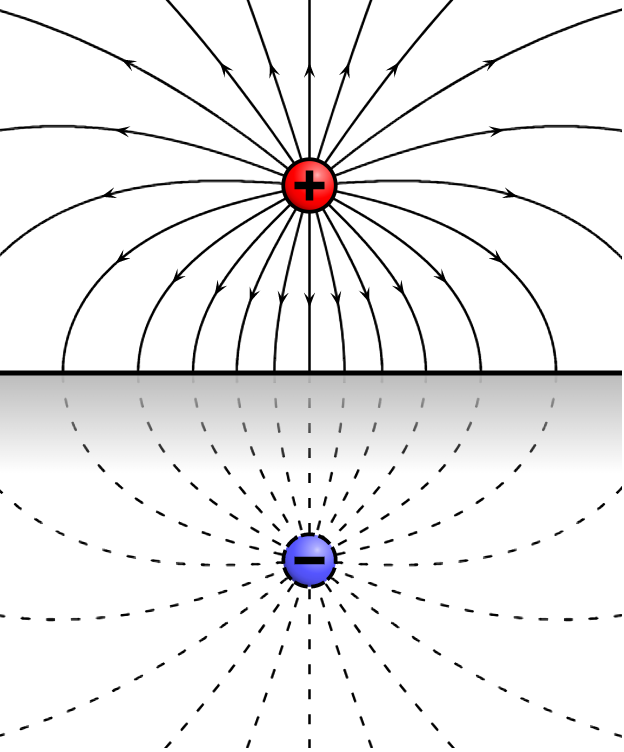
\includegraphics[scale = 0.3]{reflection}
		\caption{A dipole electric potential which vanishes at the boundary.}
	\end{center}
\end{figure}

Recall that we can physically interpret the fundamental solution $y \mapsto K(y - x)$ as the potential arising from the unit electric charge concentrated at the pole $y = x$. We want the potential to vanish on the boundary, so ``reflecting'' the charge distribution across the boundary we obtain a dipole distribution such that the two potentials arising from the oppositely charged poles cancel out at the boundary. For example, consider the upper-half space 
	\[ \HH := \{ (x, t) \in \R^d \times \R : t > 0 \}. \]
The distribution $(y, s) \mapsto K(y - x, s - t)$ is the potential of the positive unit charge at $(x, t)$, while the distribution $(y, s) \mapsto -K(y - x, t - s)$ is the potential of the negative unit charge at $(x, -t)$. Thus the Green's function of the upper-half space is 
	\[ G_\HH (x, t, y, s) := K(y - x, s - t) - K(y - x, s + t). \]
The unit normal vector on the boundary $\partial \HH$ is $\nu = (0, -1)$. The normal derivative on the boundary $s = 0$ is known as the \emph{Poisson kernel} on the upper-half space, taking the form
	\[ P_t (x - y) := \partial_\nu G_\HH (x, t, y, 0) = \frac{2}{A_d} \frac{t}{(t^2 + |x - y|^2)^{\frac{d + 1}{2}}}. \]
Observe that the Poisson kernel $\{P_t\}_t$ forms a spherically-symmetric approximation to the identity, so $P_t * \phi \to \phi$ pointwise as $t \to 0$ for continuous and bounded $\phi$. Moreover, by construction $(x, t) \mapsto P_t (x - y)$ is harmonic on the upper-half space. This proves that convolving the boundary conditions with the Poisson kernel furnishes the solution to the Dirichlet problem. 
	

\begin{theorem}[Poisson integral formula for $\HH$]
	Suppose $\phi : \partial \HH \to \R$ is bounded and continuous, then $u : \HH \to \R$ defined by the formula
		\[ u(x) := \int_{\R^d} P_t (x - y) \phi(y) d y = (P_t * \phi)(x) \]
	is the unique harmonic function extending continuously to the boundary such that $u_{|\partial \HH} = \phi$. 
\end{theorem}

Consider now the case of the ball $B \subseteq \R^d$ of radius $R > 0$ centered at the origin. Given $x \in \R^d$, define its reflection across the boundary of the ball by 
	\[ \overline x := \frac{R^2}{|x|^2} x. \]
Following the construction of the Green's function for the upper-half space, we want to place a positive unit charge at $x \in B$ and a negative unit charge at $\overline x \in \R^d \setminus B$ such that the net potential vanishes on the boundary. The Green's function of the ball $B$ is
	\[ G_B (x, y) := K(y - x) - K\left( \frac{|x|}{R}(y - \overline x)\right). \]
The unit normal vector on the boundary $\partial B$ is $\nu = y/R$. The normal derivative restricted to the boundary $|y| = R$ is known as the \emph{Poisson kernel} on the ball, taking the form 
	\[ P (x, y) := \partial_\nu G_B (x, y) =\frac{R^{d - 2} (R^2 - |x|^2)}{|x - y|^d}.  \]
As with the upper-half space, the Poisson kernel on the ball is harmonic, non-negative, and has unit mass. Integrating against boundary conditions furnishes the solution to the Dirichlet problem. 

\begin{theorem}[Poisson integral formula for ball]
	Let $B \subseteq \R^d$ be an open ball of radius $R > 0$ centered at the origin, and suppose $\phi : \partial B \to \R$ is continuous. Then $u : B \to \R$ defined by the formula
		\[ u(x) := \frac{1}{\area \partial B} \int_{\partial B} P(x, y) \phi(y) d \area (y) \]
	is the unique harmonic function extending continuously to the boundary such that $u_{|\partial B} = \phi$. 
\end{theorem}

\subsection{$C^\infty$ elliptic regularity}

When solving a linear partial differential equation distributionally, \textit{a priori} we do not know whether the solution exhibits any regularity in the strong sense. In the case of the Laplace operator, we have \textit{elliptic regularity}, the property that regularity is not ``lost'' when solving the Poisson equation. The classic example is Weyl's lemma: if the Laplacian of a distribution is smooth, then the distribution is also smooth.

\begin{theorem}[Weyl's lemma]
	Let $u \in C^\infty_c (\Omega)^*$ be a distributional solution to the Poisson equation 
		\[ \Delta u = f\]
	for $f \in C^\infty (\Omega)$. Then $u$ is smooth. 
\end{theorem}

\begin{proof}
	Fix $x \in \Omega$ and suppose $B_{5\epsilon} (x) \subseteq \Omega$. Choose a cut-off $\chi \in C^\infty_c (\Omega)$ such that $\chi \equiv 1$ on the ball $B_{4\epsilon} (x)$. Smoothness is a local property, so it suffices to show $\chi u$ is smooth at $x$. Observe that $\chi u$ defines a compactly supported distribution on $\R^d$, so we can write
		\[ \chi u = \delta_0 * (\chi u) = \Delta K * (\chi u) = K * \Delta (\chi u). \]
	Choose another cut-off $\eta \in C^\infty_c (\Omega)$ supported on $B_{3\epsilon} (x)$ and satisfies $\eta \equiv 1$ on the ball $B_{2\epsilon} (x)$. By construction, $\eta \Delta(\chi u) = \eta \Delta u = \eta f$, so we can write
		\[ \chi u = \delta_0 * (\chi u) = \Delta K * (\chi u) = K * \Delta (\chi u) = K * (\eta f) + K * (1 - \eta) \Delta (\chi u). \]
	Since $\eta f \in C^\infty_c (\R^d)$, the first term on the right is smooth. We claim that the second term on the right is smooth at $x$, which would complete the proof. Choose the final cut-off $\psi \in C^\infty_c (\R^d)$ supported in $|x| < \epsilon$ such that $\psi \equiv 1$ in a neighborhood of the origin, then 
		\[ K * (1 - \eta) \Delta (\chi u) = (\psi K) * (1 - \eta) \Delta (\chi u) + (1 - \psi) K * (1 - \eta) \Delta (\chi u).  \]
	By construction, $(1 - \psi) K \in C^\infty (\R^d)$, so the second term on the right is smooth. On the other hand, the first term on the right vanishes in a neighborhood of $x$. Recall the support of the convolution is the sum of the supports, 
		\[ \supp (\psi K) * (1 - \eta) \Delta (\chi u) \subseteq \supp (\psi K) + \supp (1 - \eta) \Delta (\chi u) \subseteq \{ x:  |x| \leq \epsilon \} + \{ x : |x - y| > 2\epsilon \}. \]
	This proves that the convolution vanishes in $B_\epsilon (x)$, completing the proof. 
\end{proof}

\begin{remark}
	This proof relied only on the fact that the fundamental solution $K$ was smooth on $\R^d \setminus 0$. That is, if $P(D)$ is a constant coefficient linear partial differential operator with fundamental solution smooth away from the origin, then it is \emph{hypoelliptic}, i.e. any distribution satisfying $P(D) u \in C^\infty (\Omega)$ must also be smooth. In fact, hypoellipticity is equivalent to the fundamental solution being smooth away from the origin. The heat operator $\partial_t - \Delta$ is an example of a non-elliptic operator which is hypoelliptic. 
\end{remark}

\section{Maximum principle}
\label{sec:max}

The \textit{strong maximum principle} is the property that a continuous function $u : \Omega \to \R$ cannot achieve a maximum on a bounded domain $\Omega \subseteq \R^d$. The \textit{weak maximum principle} follows as a direct corollary, stating that if $u$ extends continuously to the boundary, then it achieves its maximum on the boundary. As a motivating example, the class of $C^2$-convex functions, i.e. those satisfying $\nabla^2 u \geq 0$, obeys the maximum principle. Such functions also obey the differential inequality $\Delta u \geq 0$; this weaker condition turns out to be sufficient for the maximum principle. We say that an upper semi-continuous function $u : \Omega \to \overline \R$ is \emph{distributionally sub-harmonic} if 
	\[ \langle \Delta \phi, u \rangle \geq 0 \]
for all non-negative test function $\phi \in C^\infty_c (\Omega)$. If $u \in C^2 (\Omega)$ and
	\[ \Delta u \geq 0, \]
then we say $u$ is \emph{classically sub-harmonic}. Integrating by parts shows that classical sub-harmonicity implies distributional sub-harmonicity. 

\subsection{Mean value property}

Our proof of the maximum principle will rely on the following mean value characterisation of sub-harmonic functions;

\begin{theorem}[Sub-mean value property]
	Let $\Omega \subseteq \R^d$ be open, and suppose $u : \Omega \to \overline \R$ is sub-harmonic. Then for any closed ball $B \subseteq \Omega$ is a ball centered at $x_0 \in B$ we have
		\begin{align*}
			u(x_0) 
				&\leq \frac{1}{\vol B} \int_B u(y) \, dy, \\
			u(x_0)
				&\leq \frac{1}{\area \partial B} \int_{\partial B} u(y) \, d \area	.
		\end{align*}
	Conversely, if $u$ is continuous and satisfies the inequalities above for all $x_0 \in \Omega$ and sufficiently small balls $B \subseteq \Omega$ centered at $x_0$, then $u$ is sub-harmonic.
\end{theorem}

\begin{proof}
	The first inequality follows from the second by converting to spherical coordinates, so we aim towards the latter. It suffices to prove the result assuming smoothness by replacing $u$ with the convolution smoothing $u * \phi_\epsilon$ where $\phi \in C^\infty_c (|x| \leq 1)$ is non-negative and $\int \phi = 1$. Indeed, $u * \phi_\epsilon \to u$ uniformly on $B$ and, since $u$ is distributionally sub-harmonic, we have
		\[ \Delta (u * \phi_\epsilon) (x) = \int_\Omega \Delta \phi_\epsilon (x - y)\, u(y) dy \geq 0, \]
	i.e. $u * \phi_\epsilon$ is classically sub-harmonic. Assume then $u$ is smooth, we argue by a monotonicity formula, defining 
		\[ \Phi (r) := \frac{1}{\area \partial B_r (x_0)} \int_{\partial B_r (x_0)} u(y) \, d \area (y) = \frac{1}{\area \partial B_1 (0)} \int_{\partial B_1 (0)} u(x_0 + ry) \, d \area (y).  \]
	To conclude the sub-mean value property, it would suffice to show $\Phi$ is non-decreasing in $r$ since $\Phi(r) \to u(x_0)$ as $r \to 0$ by continuity of $u$. Differentiating, applying the divergence theorem and sub-harmonicity, we obtain
		\[ \Phi' (r) =  \frac{1}{\area \partial B_1 (0)} \int_{\partial B_1 (0)} y \cdot \nabla u(x_0 + ry) \, d \area (y) = \frac{1}{\area \partial B_1 (0)} \int_{B_1 (0)} \Delta u(x_0 + ry) \, dy \geq 0, \]
	as desired. 
	
	Conversely, suppose that $u$ satisfies the sub-mean value property. Then for any $\epsilon \ll 1$ such that $B_\epsilon (x) \subseteq \Omega$, we have the inequality
		\[ 0 \leq \int_{|y| \leq \epsilon} (u(x - y) - u(x)) \, dy. \]
	Let $\phi \in C^\infty_c (\Omega)$ be a non-negative test function supported on $K \subseteq \Omega$, and denote $K_\epsilon$ the $\epsilon$-neighborhood of $K$, in particular $K_\epsilon \subseteq \Omega$ for $\epsilon \ll 1$. Integrating the inequality above against $\phi$ and applying Fubini's theorem gives
		\begin{align*}
			0 
				&\leq \frac{1}{\epsilon^{2 + d}} \int_\Omega \int_{|y| \leq \epsilon} (u(x - y) - u(x)) \, \phi(x) \, dy dx = \int_{K_\epsilon} u(x) \left( \frac{1}{\epsilon^{2 + d}} \int_{|y| \leq \epsilon} (\phi(x - y) - \phi(x)) \, dy \right) \, dx.
		\end{align*}
	Consider the Taylor expansion of our test function $\phi(x - y) - \phi(x) = - \sum_j\partial_j \phi(x) y_j	 + \tfrac12 \sum_{i,j} \partial_i \partial_j \phi(x) y_i y_j + O(|y|^3)$, observing that by symmetry the integral over the first order terms vanish, the integral over the second order terms vanish off the diagonal $i \neq j$, and the integral over the third order term is controlled by $\epsilon$, i.e.
		\[ \int_{|y| \leq \epsilon} y_j  \, dy = 0, \qquad  \frac{1}{\epsilon^{2 + d}} \int_{|y| \leq \epsilon}  y_i y_j \, dy = c_d \delta_{ij}, \qquad \frac{1}{\epsilon^{2 + d}} \int_{|y| \leq \epsilon} O(|y|^3) \, dy = O(\epsilon) \]
	for some constant $c_d > 0$. Collecting our results and taking $\epsilon \to 0$, we conclude
		\[ 0 \leq \frac{c_d}{2} \int_K u(x) \Delta\phi (x) \, dx, \]
	i.e. $u$ is distributionally sub-harmonic.  	
\end{proof}

\begin{corollary}
	The class of sub-harmonic functions form a convex hull, that is, if $u, v : \Omega \to \R$ are sub-harmonic, then $\max \{ u, v \} : \Omega \to \R$ is sub-harmonic. 
\end{corollary}

\begin{proof}
	It suffices to show $\max \{u, v \}$ satisfies the sub-mean value property. Applying the sub-mean value property to $u$ and $v$, we obtain
		\begin{align*}
			 u(x_0) \leq \frac{1}{\vol B} \int_B u(y) \, dy \leq \frac{1}{\vol B} \int_B \max \{u(y), v(y) \} \, dy \\
			v(x_0) \leq \frac{1}{\vol B} \int_B v(y) \, dy \leq \frac{1}{\vol B} \int_B \max \{u(y), v(y) \} \, dy 
		\end{align*} 
	as desired. 	
\end{proof}

\begin{corollary}[Mean value property]
	Let $\Omega \subseteq \R^d$ be open, and suppose $u : \Omega \to \overline \R$ is harmonic. Then for any ball $B \subseteq \Omega$ is a ball centered at $x_0 \in B$ we have
		\begin{align*}
			u(x_0) 
				&= \frac{1}{\vol B} \int_B u(y) \, dy, \\
			u(x_0)
				&= \frac{1}{\area \partial B} \int_B u(y) \, d \area(y).
		\end{align*}
	Conversely, if $u$ is continuous and satisfies the equalities above for all $x_0 \in \Omega$ and sufficiently small balls $B \subseteq \Omega$ centered at $x_0$, then $u$ is harmonic.
\end{corollary}	

\begin{proof}
	If $u$ is harmonic, then the proof of the sub-mean value property continues to hold replacing $u$ with $-u$, which furnishes equalities in place of the inequalities. 
\end{proof}

\subsection{$C^\omega$ elliptic regularity}

One can view the mean value property as an instance of elliptic regularity. If $u$ is harmonic, then by commuting differentiation with the Laplacian, we see that $\partial_j u$ is also harmonic. Applying the mean value theorem and integration by parts gives control of a derivative by $u$ itself. Iterating furnishes control over all derivatives, more precisely,

\begin{theorem}[Cauchy estimates]
	Let $B \subseteq \R^d$ be the ball of radius $R > 0$ centered at $x_0 \in \R^d$, and suppose $u: B \to \R$ is harmonic and extends continuously to the boundary. Then
		\[ | \partial^\alpha u(x_0)| \leq \left( \frac{d |\alpha|}{R}\right)^{|\alpha|} \sup_B |u|. \]
	In particular, $u$ is real analytic. 	
\end{theorem}

\begin{proof}
	Commuting differentiation with the Laplacian, observe that $\partial^\alpha u$ is harmonic. We argue inductively; by the mean value property and the divergence theorem,   
		\[ \partial_j u (x_0) = \frac{1}{\vol B} \int_B \partial_j u  \, dy = \frac{1}{\vol B} \int_B \operatorname{div} (u \vec e_j) \, dy = \frac{1}{\vol B} \int_{\partial B} u \vec e_j \cdot \nu \, d\area. \]	
	It follows from $\area \partial B_r (x)/\vol B_r (x) = d/r$ and the triangle inequality that
		\[ |\partial_j u(x_0)| \leq \frac{d}{R} \sup_B |u| . \]	
	This proves the result for $|\alpha| = 1$. Set $m = |\alpha|$ and $\alpha_1, \dots, \alpha_m$ be a decreasing set of multi-indices $\alpha_{j} < \alpha_{j + 1}$ such that $|\alpha_j| = j$ and $\alpha_m = \alpha$. We apply the $|\alpha| = 1$ case to control $\alpha_{j + 1}$-derivatives by $\alpha_j$-derivatives on balls of radii $R/|\alpha|$. Iterating, we obtain
		\begin{align*}
			|\partial^\alpha u(x_0)|
				&\leq \left(\frac{d |\alpha|}{R} \right) \sup_{B_{R/|\alpha|} (x_0)} |\partial^{\alpha_{m - 1}} u| \leq \left(\frac{d |\alpha|}{R} \right)^2 \sup_{B_{2R/|\alpha|} (x_0)} |\partial^{\alpha_{m - 2}} u| \leq \dots \leq \left(\frac{d |\alpha|}{R} \right)^{|\alpha|} \sup_{B_{R} (x_0)} | u|
		\end{align*}
	as desired. 
\end{proof}

\begin{lemma}
	Let $\{ u_n \}_n$ be a sequence of harmonic functions on a domain $\Omega \subseteq \R^d$ converging uniformly on compact sets to $u$. Then $u$ is harmonic. 
\end{lemma}

\begin{proof}
	The mean value property is preserved under the limit, so $u$ also satisfies the mean value property, 
		\[ u(x_0) = \lim_{n \to \infty} u_n (x_0) = \lim_{n \to \infty} \frac{1}{\vol B} \int_B u_n (y) \, dy =  \frac{1}{\vol B} \int_B u (y) \, dy, \]
	for all $x_0 \in \Omega$ and closed balls $B \subseteq \Omega$ centered at $x_0$. 	
\end{proof}


\begin{theorem}[Montel's theorem]
	A family of harmonic functions $\mathcal F$ on a domain $\Omega \subseteq \R^d$ is pre-compact, i.e. every sequence has a sub-sequence converging uniformly on every compact $K \subseteq \Omega$, if and only if $\mathcal F$ is uniformly bounded. 
\end{theorem}

\begin{proof}
	We claim that $\mathcal F$ is equicontinuous on every compact $K \subseteq \Omega$. Choose $R > 0$ such that $B_{2R} (x) \subseteq \Omega$ for every $x \in K$, then by the first-order Cauchy estimate
		\[ |\nabla u (x)| \leq \frac{d}{R} \sup_B |u| \lesssim 1 \]
	uniformly in $u \in \mathcal F$ and $x \in K$. In particular, this holds for a compact neighborhood $K_\epsilon \subseteq \Omega$, so it follows from the mean value theorem that $u$ is Lipschitz continuous on $K$. By Arzela-Ascoli, for every sequence $\{u_n\}_n \subseteq \mathcal F$ there exists a sub-sequence converging uniformly on $K$.
	
	There exists a compact exhaustion $K_n \subseteq \Omega$ of the domain, i.e. $\bigcup_m K_m = \Omega$. We inductively extract sub-sequences $\{ u_{n, m} \}_n$ converging uniformly on $K_m$. The diagonal sequence $\{ u_{n, n} \}_n$ converges uniformly on every $K_n$ and moreover, since they form an exhaustion of $\Omega$, every compact $K \subseteq \Omega$. 	
\end{proof}


\subsection{Maximum principles}

We are now ready to establish the maximum principle for sub-harmonic functions and its consequences. 

\begin{theorem}[Strong maximum principle]
	Let $\Omega \subseteq \R^d$ be open and connected and $u: \Omega \to \R$ be sub-harmonic. If $u$ achieves its maximum, i.e. there exists $x_0 \in \Omega$ such that
		\[ u(x_0) = \sup u(\Omega), \]
	then $u$ is constant. 
\end{theorem}

\begin{proof}
	We know from upper semi-continuity that the level set $u = \sup u (\Omega)$ is closed, so it suffices by connectivity to show it is also open. Let $B \subseteq \Omega$ be an open ball centered at $x_0$, then by the sub-mean value property and $u(x_0) \geq u(y)$ we have
		\[ 0 \geq \int_B (u(x_0) - u(y)) \, dy = \int_B |u (x_0) - u(y)| \, dy. \]
	It follows from semi-continuity that $u \equiv u(x_0)$ on the ball $B$, as desired. 
\end{proof}

\begin{corollary}[Weak maximum principle]
	Let $\Omega \subseteq \R^d$ be open and $u : \Omega \to \R$ be sub-harmonic. If $u$ is bounded and extends continuously to the boundary, then it achieves its maximum on the boundary, i.e.
		\[ \sup u (\partial \Omega) = \sup u(\Omega). \]
\end{corollary}

\begin{corollary}[Comparison principle]
	Let $\Omega \subseteq \R^d$ be open, and suppose $u, h: \Omega \to \R$ are sub-harmonic and harmonic respectively extending continuously to the boundary. If $u \leq h$ on the boundary $\partial B$, then $u \leq h$ on the entire domain $\Omega$. 	
\end{corollary}	

\begin{proof}
	The difference $u - h$ is sub-harmonic on $\Omega$ extending continuously to the boundary, so it obeys the weak maximum principle, i.e. the maximum is on the boundary. Since $u - h \leq 0$ on the boundary $\partial \Omega$, we have $u - h \leq 0$ on the entire domain $\Omega$.
\end{proof}

\begin{theorem}[Lindelof maximum principle]
	Let $\Omega \subseteq \R^d$ be open and bounded, and suppose $u : \Omega \to \overline\R$ be sub-harmonic. Then 
		\[ \sup u(\Omega) = \sup_{x \in \partial \Omega} \limsup_{y \to x} u(y). \]
	Furthermore, if $u$ is bounded above and $F \subseteq \partial\Omega$ is finite, then 
		\[ \sup u(\Omega) = \sup_{x \in \partial \Omega \setminus F} \limsup_{y \to x} u(y). \]	
\end{theorem}

\begin{proof}
	Since $\Omega$ is bounded, we can choose a maximising sequence $\{y_n\}_n \subseteq \Omega$ converging to $x \in \overline \Omega$. If $x \in \partial \Omega$, we have proven 
		\[ \sup u(\Omega) = \sup_{x \in \partial \Omega} \limsup_{y \to x} u(y). \]
	Otherwise $x \in \Omega$, which by the strong maximum principle implies $u \equiv \sup u(\Omega)$ on the connected component containing $x$, and again the equality above holds. 
	
	Suppose now $u$ is bounded above. For $\epsilon > 0$, define
		\[ v_\epsilon (y) := u(y) - \epsilon \sum_{x \in F} K(y - x), \]
	where $K$ is the fundamental solution. Note that $K(y - x) \to \infty$ as $y \to x$, so since $u$ is bounded above we have $v_\epsilon (y) \to -\infty$ as $y \to x$. It follows that 
		\begin{align*}
			\sup v_\epsilon (\Omega)
				&\leq \sup_{x \in \partial \Omega} \limsup_{y \to x} v_\epsilon (y) \leq \sup_{x \in \partial \Omega \setminus F} \limsup_{y \to x} v_\epsilon (y).
		\end{align*}
	In the case $d = 2$, we write
		\[ \sup_{x \in \partial \Omega \setminus F} \limsup_{y \to x} v_\epsilon (y) \leq \sup_{x \in \partial \Omega \setminus F} \limsup_{y \to x} u(y) + \epsilon \log (1 + \operatorname{diam} \Omega). \]
	In the case $d = 3$, using $K \geq 0$ we write
		\[ \sup_{x \in \partial \Omega \setminus F} \limsup_{y \to x} v_\epsilon (y) \leq \sup_{x \in \partial \Omega \setminus F} \limsup_{y \to x} u (y). \]	
	As $v_\epsilon \to u$ pointwise taking $\epsilon \to 0$, we conclude the result. 
\end{proof}	

\begin{remark}
	The first Lindelof maximum principle fails when the domain is not bounded; let $\mathbb H \subseteq \R^2$ be the upper-half space $y > 0$ and define $u : \HH \to \R$ by $u(x, y) := y$. Clearly the maximum is not achieved on the boundary $y = 0$. The second Lindelof maximum principle fails when $u$ is not bounded above; let $\DD \subseteq \C$ be the unit disc and define $u: \DD \setminus 0 \to \R$ by $u(z) := - \log |z|$. Then the result fails taking $F = \{0\}$ and noting $u$ vanishes on $\partial \DD$. 
\end{remark}



\begin{theorem}[Harnack's inequality]
	Let $\Omega \subseteq \R^d$ be open and connected, and suppose $u: \Omega \to [0, \infty)$ is a non-negative harmonic function. Then for any $U \Subset \Omega$ which is open and connected, there exists a constant $C(\Omega, U) > 0$ such that
		\[ \sup u( U) \leq C(\Omega, U) \inf ( U). \]
	In particular, if $u(x) = 0$ for some $x \in \Omega$, then $u \equiv 0$. 		
\end{theorem}

\begin{proof}
	It suffices to show
		\[ u(a) \leq C(\Omega, U) u(b) \]
	for any $a, b \in U$. Since $U$ has compact closure in $\Omega$, there exists $r > 0$ such that $B_{4r} (x) \subseteq \Omega$ for all $x \in U$, and a finite cover of $\Omega$ by the balls $B_r (x)$. We claim that Harnack's inequality holds on balls, 
		\[ \sup u (B_r (x)) \leq 3^d \inf u (B_r (x)). \]
	Fix $a, b \in B_r (x)$, then by the mean value property
		\begin{align*}
			u(a) 
				&= \frac{1}{\vol B_r (a)} \int_{B_r (a)} u(y) \, dy \\
				&\leq \frac{1}{\vol B_r (a)} \int_{B_{3r} (b)} u(y) \, dy =\frac{\vol B_{3r} (b) }{\vol B_r (a)} u(b) = 3^d u(b),
		\end{align*}		
	where the inequality follows from non-negativity of $u$ and $B_r (a) \subseteq B_{3r} (b) \subseteq \Omega$. This proves the claim. To extend Harnack's inequality to $U$, we remark that any two points $a, b \in U$ can be connected by a continuous path covered by the balls $B_r (x)$ in the finite cover. Iterating Harnack's inequality on these balls along the path, we obtain
		\[ u(a) \leq (3^d)^{\text{\# of balls}} u(b), \]
	completing the proof. 	
\end{proof}

\begin{remark}
	The constant $C(\Omega, U)$ does not depend on the choice of harmonic function $u$. Thus Harnack's inequality states that positive harmonic functions are controlled solely by the geometry of their domain. 
\end{remark}


\begin{corollary}[Harnack convergence theorem]
	Let $\Omega \subseteq \R^d$ be open and connected, and suppose $u_n : \Omega \to \R$ is an increasing sequence of harmonic functions such that $\sup_n u_n (x_0) < \infty$ for some $x_0 \in \Omega$. Then $\{u_n\}_n$ converges uniformly on compact sets to a harmonic function. 
\end{corollary}

\begin{proof}
	Without loss of generality, let $K \subseteq \Omega$ be compact such that $x_0 \in \Omega$. Since the sequence is increasing, $u_n - u_m \geq 0$ for all $n \geq m$. By Harnack's inequality and monotone convergence, 
		\[ 0 < \sup_K (u_n - u_m) \lesssim \inf_K (u_n - u_m) \leq u_n (x_0) - u_m (x_0) \overset{n, m \to \infty}{\longrightarrow} 0. \]
	This proves $\{u_n\}_n$ converges uniformly to some $u: \Omega \to \R$ on every compact $K$. In particular, each $u_n$ satisfies the mean value property, so passing to the limit, it follows that $u$ also satisfies the mean value property and is therefore harmonic. 
\end{proof}	



\subsection{Perron's method}

Consider the Dirichlet problem
	\begin{align*}
		\Delta u
			&= 0, \\
		u_{|\partial \Omega} 
			&= \phi	
	\end{align*}
on an open bounded domain $\Omega \subseteq \R^d$ for continuous boundary values $\phi : \partial \Omega \to \R$. We construct a suitable candidate for the solution to the Dirichlet problem via the maximum principle. A continuous sub-harmonic function $v : \Omega \to \R$ is a \emph{sub-solution} if 
	\[ \limsup_{y \to x} v(y) \leq \phi(x) \]
for all $x \in \partial \Omega$. The \emph{Perron solution} $u: \Omega \to \R$ is defined as the pointwise maximum over all sub-solutions, 
	\[ u (x) := \sup\{ v(x) : \text{$v$ is a sub-solution} \}. \]
We claim $u$ solves the Dirichlet problem for sufficiently regular domains. Note first that $u$ is well-defined, i.e. sub-solutions exist and $u$ is bounded. Indeed, the boundary $\partial \Omega$ is compact and so the boundary values $\phi$ are bounded. The constant function equal to the lower bound is a sub-solution, and from the Lindelof maximum principle $u$ is bounded above by 
	\[ \sup v(\Omega) = \sup_{x \in \partial \Omega} \limsup_{y \to x} v(y) \leq \sup \phi(\partial \Omega) \]
whenever $v$ is a sub-solution. We now turn to showing the Perron solution is harmonic;

\begin{lemma}
	Let $\Omega \subseteq \R^d$ be open, and suppose $u: \Omega \to \R$ is continuous and sub-harmonic. If $h : \overline B \to \R$ is a harmonic function on the ball $\overline B \subseteq \Omega$ such that $u_{|\partial B} = h_{|\partial B}$, then the \emph{harmonic lift} $u_B : \Omega \to \R$ defined by
		\[ u_B (x)
			:=
			\begin{cases}
				u(x), 		&\text{if }x \not\in B, \\
				h(x), 		&\text{if }x \in \overline B 
			\end{cases}
		 \]
	is sub-harmonic and $u \leq u_B$.  
\end{lemma}

\begin{proof}
	From the comparison principle we see that $u \leq u_B$. Fix a closed ball $D \subseteq \Omega$ centered at $x_0 \in \Omega$ and let $g : D \to \R$ be the harmonic function agreeing with $u_B$ on the boundary. We claim $u_B \leq g$ on the ball $D$; it would follow that $u_B$ satisfies the sub-mean value property,
		\[ u_B(x_0) \leq g(x_0) = \frac{1}{\area \partial D} \int_{\partial D} u_B (y) d \area (y), \]
	i.e. $u_B$ is sub-harmonic. Since $u \leq u_B \leq g$ on the boundary $\partial D$, the comparison principle implies $u \leq g$ on the entire ball $D$. This proves $u_B \leq g$ on $D \setminus B$. It remains to consider the region $D \cap B$. Note $g - h$ is harmonic, so it achieves its maximum over $D \cap B$ on the boundary, which consists of two components $\partial D \cap B$ and $\partial B \cap D$. On the former $g = u_B = h$, on the latter, $h = u$, so we are done. 
\end{proof}

\begin{theorem}
	Let $\Omega \subseteq \R^d$ be open and bounded, and suppose $\phi : \partial \Omega \to \R$ is continuous. Then the Perron solution to the corresponding Dirichlet problem is harmonic. 
\end{theorem}

\begin{proof}
	Fix $x_0 \in \Omega$ and choose a sequence of sub-solutions $\{ v_n \}_n$ such that $v_n (x_0) \to u(x_0)$. We can assume the sequence is increasing and bounded below by $\inf \phi$ by replacing with the pointwise maximum	 
		\[ x \mapsto \max \{ v_1(x), \dots, v_n (x), \inf \phi (\partial \Omega) \}, \]
	as sub-solutions are closed under pointwise maximums. Furthermore, the harmonic lift $(v_n)_B$ on a ball $B \subseteq \Omega$ centered at $x_0$ is a sub-solution since it is sub-harmonic and the boundary values remain unchanged. Set
		\[ v(x) := \lim_{n \to \infty} (v_n)_B (x). \]
	By Harnack's convergence theorem, $v$ is harmonic in $B$. Moreover, $v(x_0) = u(x_0)$ by the comparison principle,
		\[ u(x_0) \geq (v_n)_B (x_0) \geq v_n (x_0) \overset{n \to \infty}{\longrightarrow} u(x_0). \]
	Showing $u \equiv v$ on $B$ completes the proof. By construction, $v \leq u$, so assume towards a contradiction there exists $x_1 \in B$ such that $v(x_1) < u(x_1)$. Repeating the beginning of the proof, we can find a bounded non-decreasing sequence of sub-solutions $\{ w_n \}_n$ such that $w_n (x_1) \to u(x_1)$. Define
		\[ w(x) := \lim_{n \to \infty} (\max \{ v_n, w_n \})_B (x). \]
	By Harnack's convergence theorem, $w$ is harmonic in $B$. Moreover, $v(x_0) = w(x_0)$ by the comparison principle, 
		\[ v(x_0) \leq w(x_0) \leq u(x_0) = v(x_0). \]
	Note $v - w$ is a non-positive harmonic function on $B$ vanishing at $x_0$, so by the weak maximum principle $v \equiv w$ on $B$. However $w(x_1) = u(x_1)$ and, by assumption, $v(x_1) \neq u(x_1)$, a contradiction. 		
\end{proof}

\section{Energy method}

The methods discussed thus far do not have robust generalisations outside the realm of constant-coefficient linear partial differential equations. We will instead appeal to functional analysis, where the natural function spaces to consider are the Sobolev spaces $W^{1, p} (\Omega)$ for $1 < p < \infty$, in which case the boundary conditions need to be taken in the sense of traces. Suppose then $\Omega \subseteq \R^d$ is a $C^1$-domain, and let $f \in W^{-1, p} (\Omega)$ and $\phi \in W^{1-1/p, p} (\partial \Omega)$, then the Dirichlet problem takes the form
	\begin{alignat*}{2}
		\Delta u
			&= f, \qquad  && \text{on } \Omega, \\
		u
			&= \phi,	\qquad && \text{on } \partial \Omega.
	\end{alignat*} 
We refer to solutions $u \in W^{1,p} (\Omega)$ as \emph{weak solutions}. In view of Sobolev embedding, weak solutions are in fact classical solutions provided sufficient regularity or integrability. 

\subsection{Existence and uniqueness}

We can reduce to solving the Dirichlet problem with homogeneous boundary conditions by choosing an extension of the boundary values $g \in W^{1, p} (\Omega)$, that is, $g_{|\partial \Omega} = \phi$. Indeed, suppose $v \in W^{1, p}_0 (\Omega)$ solves
\begin{alignat*}{2}
		\Delta v
			&= f + \Delta g, \qquad  && \text{on } \Omega, \\
		v
			&= 0,	\qquad && \text{on } \partial \Omega,
	\end{alignat*} 
then $u = v - g$ solves the original Dirichlet problem. The space $W^{1, p}_0 (\Omega)$ is reflexive and dual to the negative Sobolev space $W^{-1, p} (\Omega) = (W^{1, p}_0 (\Omega))^*$. It follows by duality and self-adjointness of the Laplace operator that uniqueness of a solution to the Dirichlet problem implies existence of a solution. More precisely, we record the following general lemma:

\begin{lemma}[Existence-uniqueness duality]
	Let $P : X \to Y$ be a linear operator between Banach spaces, and denote $P^* : Y^* \to X^*$ its adjoint, then 
		\begin{itemize}
			\item uniqueness furnishes existence for the dual problem, i.e. if $||u||_X \lesssim ||Pu||_Y$, then $\Im P^* = X^*$,
			\item existence furnishes uniqueness for the dual problem, i.e. if $\Im P = Y$, then $||v||_{Y^*} \lesssim ||P^* v||_{X^*}$. 
		\end{itemize}
	In particular, if $X$ is reflexive, then the a priori estimate furnishes existence and uniqueness for the problem $Pu = f$. 	
\end{lemma}

\begin{theorem}[Energy estimate]
	Let $\Omega \subseteq \R^d$ be a $C^1$-domain, and suppose $f \in W^{-1,p} (\Omega)$. Then a solution $u \in W^{1, p}_0 (\Omega)$ to the Dirichlet problem
		\begin{alignat*}{2}
		\Delta u
			&= f, \qquad  && \text{on } \Omega, \\
		u
			&= 0,	\qquad && \text{on } \partial \Omega,
	\end{alignat*} 
	satisfies the energy estimate
		\[ || u||_{W^{1, p}_0} \lesssim || f ||_{W^{-1, p}}. \]
	In particular, there exists a unique weak solution to the Dirichlet problem. 	
\end{theorem}

\begin{proof}
	Choose a sequence $\{ u_n \}_n \subseteq C^\infty_c (\Omega)$ such that $u_n \to u$ in $W^{1 ,p}_0 (\Omega)$. Moreover, by duality $\Delta u_n \to f$ in $W^{-1, p} (\Omega)$. The operator $\partial_j/|\nabla|$ is a Mikhlin multiplier, so it is bounded on $L^p (\R^d)$ and thus
		\[ || \partial_j u_n ||_{L^p (\R^d)} \lesssim || |\nabla| u_n||_{L^p (\R^d)} \sim || \Delta u_n||_{W^{-1, p} (\Omega)} . \]
	Summing in $j$, passing to the limit and applying the Poincare inequality on the left, we conclude
		\[ || u ||_{W^{1, p}_0} \lesssim || f||_{W^{-1, p}}. \]	
	This completes the proof. 	
\end{proof}

\begin{remark}
	It is illustrative to consider the case $p = 2$ which can be proven using elementary tools. Integrating the equation against $u$ and integrating by parts, we can write
		\[ \int_\Omega u f \, dx = \int_\Omega u \Delta u \, dx = - \int_\Omega |\nabla u|^2 \, dx. \]
	Applying duality to the left and the Poincare inequality to the right, we obtain
		\[ ||u||_{H^1_0}^2 \sim ||u||_{\dot H^1}^2 \leq || u ||_{H^1_0} ||f||_{H^{-1}}. \]	
\end{remark}

\subsection{$W^{k, p}$ elliptic regularity}

The energy estimate \textit{a priori} only furnishes solutions to the Dirichlet problem in the weak sense. Ideally, we would like to know if $u$ admits higher order weak derivatives, which by Sobolev embedding would furnish strong derivatives and imply the solution is in fact a classical solution. We appeal to elliptic regularity, claiming that if $f \in W^{k, p} (\Omega)$, then solving the Poisson equation
	\[ \Delta u = f \]
for $u \in W^{1, p} (\Omega)$ does not ``lose'' regularity in the sense that any solution satisfies $u \in W^{k + 2, p} (\Omega)$. This would follow from an argument similar to the proof of the energy estimate provided we knew \textit{a priori} our solution had the desired regularity. We instead replace the derivative operators with the difference quotient
	\[ D^h_i u (x) := \frac{u(x + h \vec e_i) - u(x)}{h}. \]


\begin{theorem}[$W^{k, p}_{\loc}$ elliptic regularity]
	Let $\Omega \subseteq \R^d$ be a domain. For $f \in W^{k, p} (\Omega)$, suppose that $u \in W^{1, p} (\Omega)$ is a solution to Poisson's equation
		\[ \Delta u  = f. \]
	Then $u \in W^{k + 2, p}_{\loc} (\Omega)$ and for each $V \Subset \Omega$ we have the estimate	
		\[ || u||_{W^{k + 2, p} (V)} \lesssim_V ||f||_{W^{k, p} (\Omega)} + ||u||_{W^{k, p}(\Omega)}. \]
\end{theorem}

\begin{proof}
	We argue inductively, considering first the case $k = 0$. Let $V \Subset W \Subset \Omega$, and choose a non-negative cut-off $\chi \in C^\infty_c (W)$ satisfying $\chi \equiv 1$ on $V$. The operator $D^h_i \langle \nabla \rangle/(\Delta + 1)$ is a Mikhlin multiplier uniformly in $h$, so it is bounded on $L^p (\R^d)$. In particular, 
		\begin{align*}
			 ||D^h_i \langle \nabla \rangle (\chi u)||_{L^p (\R^d)} 
			 	&\lesssim || (\Delta + 1) (\chi u)||_{L^p (\R^d)} \\
			 	&\leq ||\Delta (\chi u)||_{L^p (\R^d)} + ||\chi u||_{L^p (\R^d)}  \lesssim_\chi ||f||_{L^p (\Omega)} + ||u||_{L^p (\Omega)}
		\end{align*}
	uniformly in $h$. It follows that $\langle \nabla \rangle (\chi u) \in W^{1, p} (W)$ and
		\[  \sum_{|\alpha| = 1, 2} ||\partial^\alpha u||_{L^p (V)} \lesssim \sum_i ||\partial_i \langle \nabla \rangle  (\chi u)||_{L^p (W)} \lesssim ||f||_{L^p (\Omega)} + ||u||_{L^p (\Omega)}. \]
	This proves the base case. Assume the result holds for $k$, then following the same multiplier argument and applying the induction hypothesis we obtain
	\begin{align*}
			 ||D^h_i \langle \nabla \rangle^{k + 1} (\chi u)||_{L^p (\R^d)} 
			 	&\lesssim || (\Delta + 1) \langle \nabla \rangle^k (\chi u)||_{L^p (\R^d)} \\
			 	&\leq ||\Delta (\chi u)||_{W^{k, p} (\R^d)} + ||\chi u||_{W^{k, p}(\R^d)}  \lesssim_\chi ||f||_{L^p (\Omega)} \lesssim_\chi ||f||_{W^{k, p} (\Omega)} + ||u||_{L^p (\Omega)}
		\end{align*}	 
	uniformly in $h$. It follows that $\langle \nabla \rangle^{k + 1} (\chi u) \in W^{1, p} (W)$ and 
		\[ \sum_{1 \leq |\alpha| \leq k + 2} ||\partial^\alpha u||_{L^p (V)} \lesssim \sum_i ||\partial_i \langle \nabla \rangle^{k + 1} (\chi u)||_{L^p (W)} \lesssim || f||_{W^{k, p} (\Omega)} + ||u||_{L^p (\Omega)}. \]	
	This completes the proof. 		
\end{proof}

\begin{remark}
	By Sobolev embedding, it follows from $k > d/2$ that $f \in C_{\loc} (\Omega)$ and $u \in C^2_{\loc} (\Omega)$, so $u$ is classical solution to Poisson's equation. 
\end{remark}

\section{Dirichlet's principle}

For $f \in H^{-1} (\Omega)$, define the \emph{Dirichlet energy} $E : H^1_0 (\Omega) \to \overline \R$ by 
	\[ E[u] := \frac12 ||u||_{\dot H^1} + \langle u, f \rangle = \frac12 \int_\Omega |\nabla u|^2 \, dx + \int_\Omega u f \, dx. \]
Dirichlet's principle states that minimising the energy is equivalent to solving the Dirichlet problem with homogeneous boundary conditions. This is an example of \textit{variational calculus}, and we say that the Poisson equation arises as the \textit{Euler-Lagrange equation} of the Lagrangian $L(x, u, \nabla u) = |\nabla u|^2 + u f$. 

\begin{theorem}[Dirichlet's principle]
	Let $\Omega \subseteq \R^d$ be a $C^1$-domain, and suppose $f \in H^{-1} (\Omega)$. Then $u \in H^1_0 (\Omega)$ solves the Dirichlet problem	
		\begin{alignat*}{2}
		\Delta u
			&= f, \qquad  && \text{on } \Omega, \\
		u
			&= 0,					\qquad && \text{on } \partial \Omega,
	\end{alignat*} 
	if and only if it minimises the Dirichlet energy, 
		\[ E[u] = \min_{v \in H^1_0 (\Omega)} E[v].  \]
\end{theorem}	

\begin{proof}
	Suppose $u$ is a minimiser, then for any test function $\phi \in C^\infty_c (\Omega)$ define $e: \R \to \R$ by
		\[ e(t) := E[u + t\phi]. \]
	By construction, $e$ is minimised at $t = 0$, so writing $|\nabla (u + tv)|^2 = |\nabla u|^2 + 2t \nabla u \cdot \nabla \phi + t^2 |\nabla \phi|^2$, differentiating under the integral sign, and integrating by parts, we obtain 
		\begin{align*}
			0
				= \frac{d}{dt} \Big|_{t = 0} e 
				&= \int_\Omega \nabla u \cdot \nabla \phi \, dx + \int_\Omega f \phi\, dx = \int_\Omega (f- \Delta u) \, \phi \, dx.
		\end{align*}	
	Since $\phi$ was arbitrary, we conclude $\Delta u = f$ in the sense of distributions, thereby solving the Dirichlet problem. 
	
	Suppose $u$ is a solution to the Dirichlet problem, and let $v \in H^1_0 (\Omega)$, then testing $0 = \Delta u - f$ against $u - v$ and integrating by parts gives
		\begin{align*}
			 0 = \int_\Omega (\Delta u - f) (u - v) \, dx 
				&= \int_\Omega f ( u - v) \, dx - \int_\Omega \nabla u \cdot \nabla (u - v) \, dx \\
				&= \int_\Omega u f \, dx - \int_\Omega v f \, dx - \int_\Omega |\nabla u|^2 \, dx + \int_\Omega \nabla u \cdot \nabla v \, dx.
		\end{align*}		
	By Cauchy-Schwartz and the arithmetic-geometric mean inequality, $\nabla u \cdot \nabla v \leq \tfrac12 |\nabla u|^2 + \tfrac12 |\nabla v|^2$. Rearranging above and applying this inequality, we obtain
		\[ \int_\Omega |\nabla u|^2 \, dx - \int_\Omega uf \, dx \leq \tfrac12 \int_\Omega |\nabla u|^2 \, dx + \tfrac12 \int_\Omega |\nabla v|^2 \, dx - \int_\Omega v f \, dx.  \]	
	Rearranging gives $E[u] \leq E[v]$. Since $v$ was arbitrary, we conclude $u$ is a minimiser of the Dirichlet energy. 	
\end{proof}

\begin{theorem}[Existence and uniqueness of a minimiser]
	Let $\Omega \subseteq \R^d$ be a $C^1$-domain, and suppose $f \in H^{-1} (\Omega)$. Then there exists a unique solution $u \in H^1_0 (\Omega)$ to the Dirichlet energy $E: H^1_0(\Omega) \to \overline \R$. 
\end{theorem}

\begin{proof}
	Uniqueness follows from strict convexity of the energy. Indeed, $E$ is the sum of a strictly convex functional $u \mapsto ||u||_{\dot H^1}^2$ and a linear functional $u \mapsto \langle u, f\rangle$, so if $u, v \in H^1_0 (\Omega)$ are distinct minimisers, then 
		\[ E[\tfrac12 u + \tfrac12 v] < \frac{E[u] + E[v]}{2} = \min_{w \in H^1_0} E[w], \]
	a contradiction. 	
	
	Existence follows from coercivity and weak lower semi-continuity of the energy on the weakly compact space $H^1_0 (\Omega)$. We first show coercivity; by duality and the Poincare inequality, the energy is bounded below by 
		\[ E[u] \geq \frac12 ||u||_{\dot H^1}^2 - ||u||_{H^1_0} ||f||_{H^{-1}} \gtrsim ||u||_{H^1_0}^2 - ||u||_{H^1_0} ||f||_{H^{-1}}. \]
	It follows that $E[u] \to \infty$ whenever $||u||_{H^1_0} \to \infty$. In particular, a minimising sequence $\{ u_k \}_k \subseteq H^1_0 (\Omega)$ of the energy must be bounded. We can therefore pass to a sub-sequence such that $u_k \rightharpoonup u$ for some $u \in H^1_0 (\Omega)$. By showing weak lower semi-continuity, that is, 
		\[ E[u] \leq \liminf_{k \to \infty} E[u_k] ,\]
	we can conclude $u$ is the minimiser. By the arithmetic-geometric mean inequality, $|y|^2 \geq |x|^2 + 2 x \cdot (y - x)$ for all $x,y \in \R^d$. Hence
		\[ E[u_n] \geq E[u] + \int_\Omega \nabla u \cdot (\nabla u_n - \nabla u) \, dx + \int_\Omega (u - u_n ) f  \, dx \overset{n \to \infty}{\longrightarrow} E[u],  \]
	where by construction $u_n \rightharpoonup u$ in $H^1_0 (\Omega)$ and $\nabla u_n \rightharpoonup \nabla u$ in $L^2 (\Omega)$. This completes the proof.
\end{proof}


\bibliographystyle{alpha}
\bibliography{biblio}

\end{document}